\section{Implementation}
\label{sec:system}

This section describes the implementation of \scout
as shown in \myfigure{\ref{fig:system_design}}.
We implement the system in Python with
scikit-learn~\cite{scikit-learn} for machine learning libraries and
Boto 3~\cite{boto3} for interacting with Amazon web services.


\begin{figure}[!htbp]
 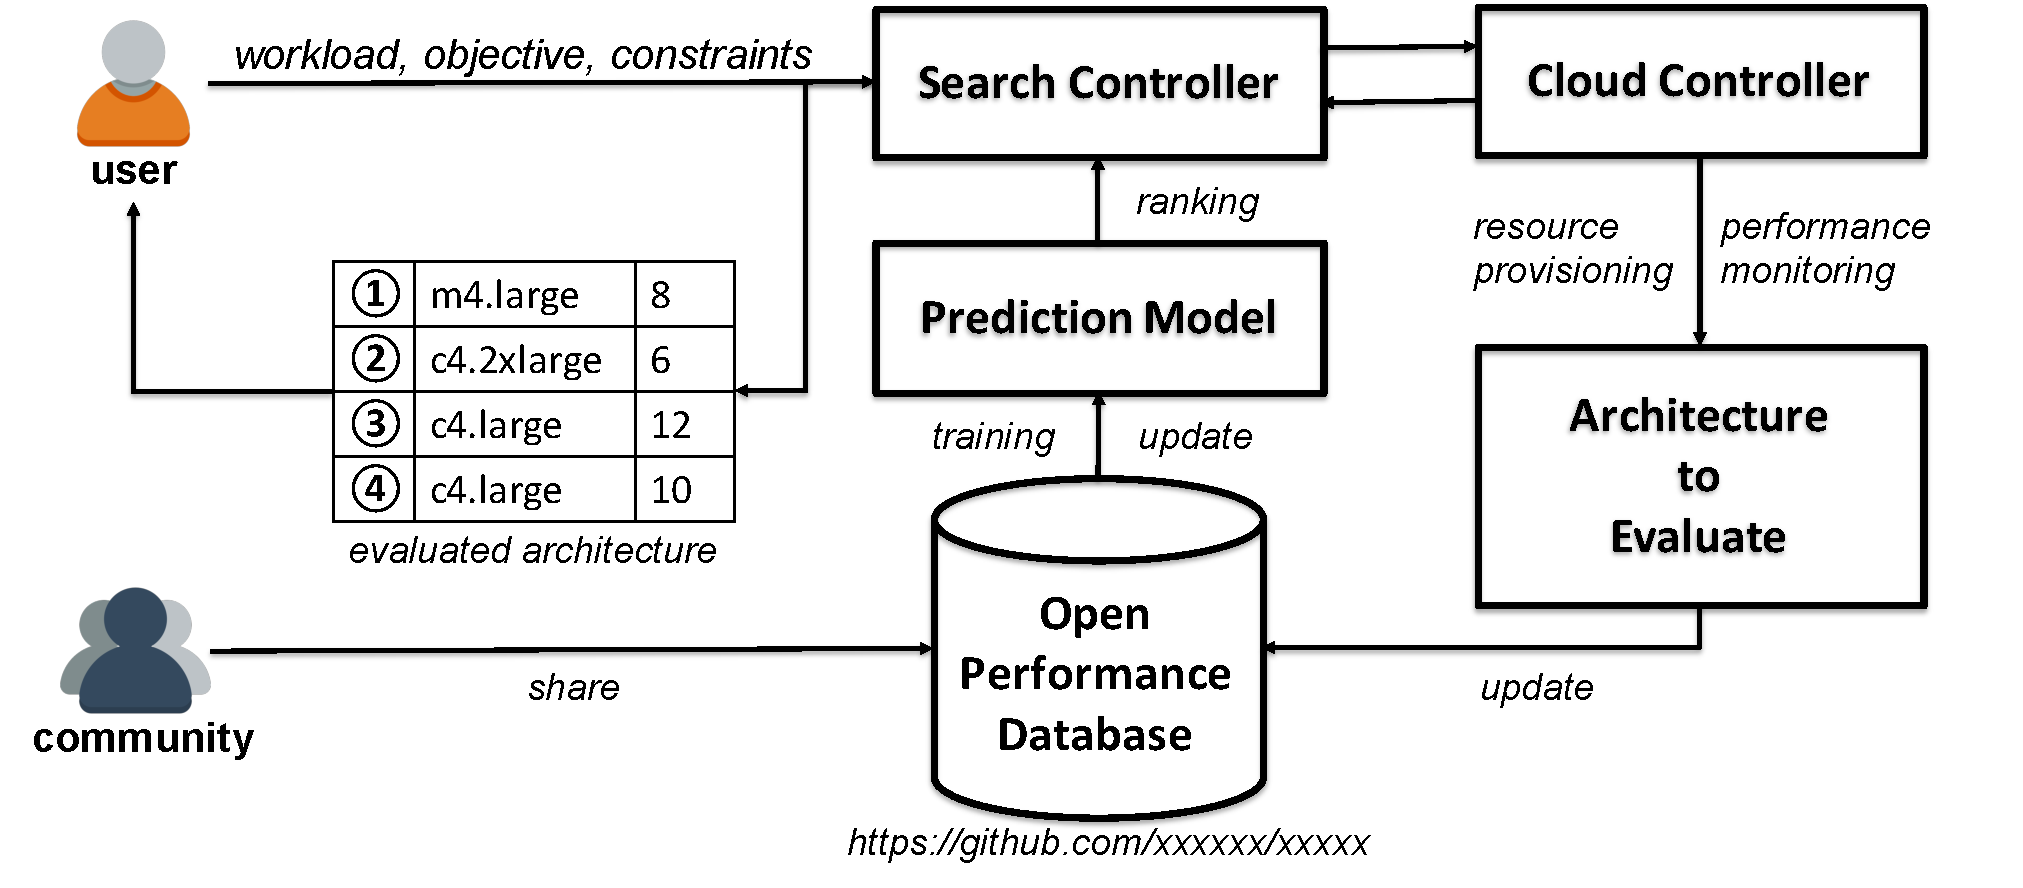
\includegraphics[width=.8\textwidth]{figures/system_design_blind.pdf}
 \centering
 \caption{\small{\textbf{\scout's implementation.}
 }}
 \label{fig:system_design}
\end{figure}


\begin{itemize}
\item \textbf{Search Controller.}
This is the entry point to use \scout.
A user submits a workload along with performance and cost objectives.
The user can also specify constraints such as maximum execution time,
maximum cost budget and the range of cluster sizes, etc.
The performance of \scout is not heavily affected by
the initial architectural configurations.
For evaluations, \scout randomly selects one configuration.
The search controller forwards the workload and the selected configuration
to the cloud controller.
Once the selected configuration is evaluated,
the search controller is notified and determines
the next configuration to evaluate.
\scout selects the configuration that, according to the model, has the
greatest likelihood of improving performance.
% The probability information is provided by the prediction model.
This optimization process stops when the objective is fulfilled or
when the evaluation budget is expended.

\item \textbf{Prediction Model.}
We can use a probabilistic classifier to derive the probability distribution
over prediction classes~\cite{friedman2001elements}.
Possible choices include, but are not limited to,
Logistic Regression, Gaussian Process, Random Forests and neural networks
~\cite{breiman2001random,friedman2001elements}.
\scout uses \emph{ExtraTree}
to train a classification model
for deriving relative ordering (to determine better configurations)
because \emph{ExtraTree} is more efficient and reliable
% to cope -- check this. does it still make your point?
with
numerical performance data~\cite{geurts2006extremely}.

\item \textbf{Cloud Controller.}
The cloud controller bridges the search controller and cloud platforms.
The controller is responsible for running the workload
with a specific architectural configuration.
\scout currently supports AWS but easily can be extended
to other cloud platforms.
For each evaluation, the cloud controller monitors the execution time and
collects low-level performance information.
We use the \emph{Sysstat} package on Linux for system monitoring~\cite{sysstat}.
Since we collect only generic performance metrics, other monitoring tools
should work as well.
We choose a five-second sampling period.
Each sample has 72 metrics from
CPU, memory, cache, disk and network components.
These numbers are then aggregated from various-size
samples (per node) and nodes (per cluster).
We follow the similar process of feature transformation
as described in~\cite{Hsu2016,Hsu2018Arrow}.

\item \textbf{Open Performance Database.}
Performance data is hard to find.
We believe sharing data can greatly advance the research
on CAT.
Moreover, cloud users benefit from the performance database because
they are able to learn the workload performance on
different architecture configurations, which are very expensive
to obtain.

\end{itemize}